\begin{figure}
    \begin{center}
    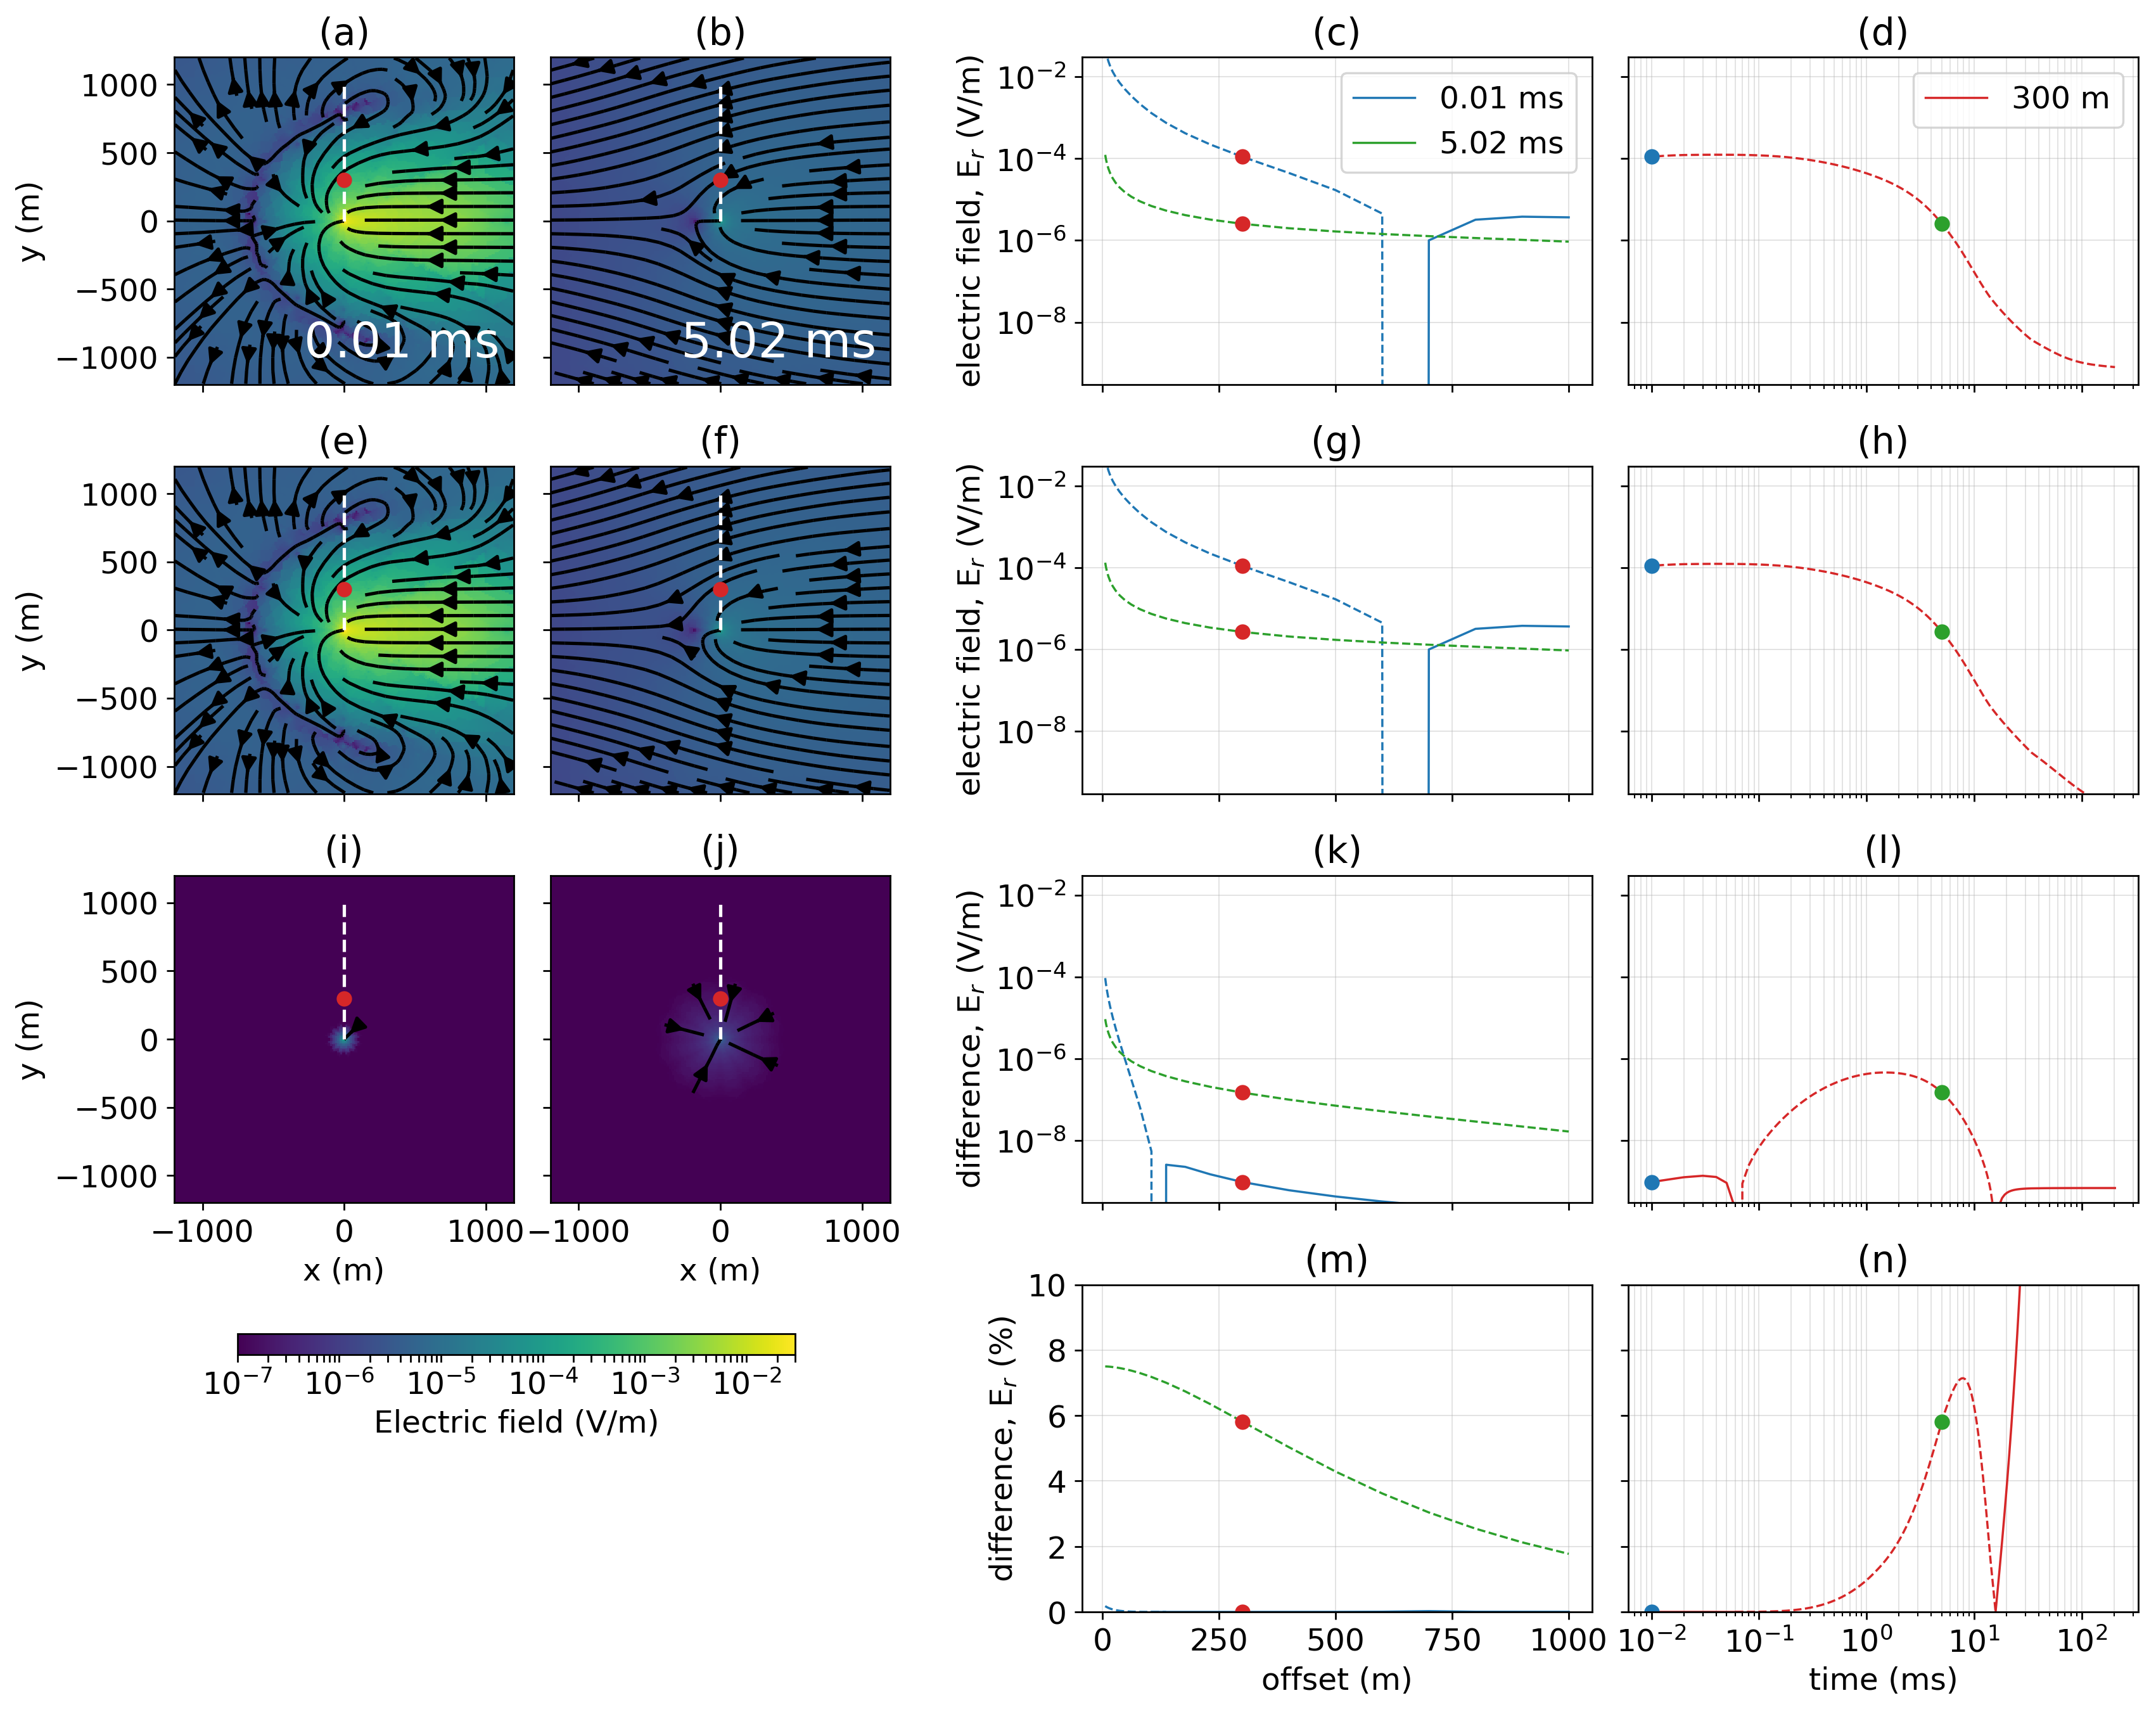
\includegraphics[width=\textwidth]{figures/em_casing/surface_e_fields_approx_casing.png}
    \end{center}
\caption{
    Simulated electric field at the surface of the earth, as was presented in \ref{fig:surface_e_fields_overview}.
    The top row (a -- d) are the data simulated with the true, conductive casing.
    The second rows (e -- h) are the data
    simulated with the solid cylinder approximating the well.
    The third row (i -- l) is the difference (approximate minus true),
    and the fourth row (m and n) show the difference as a percentage of the true solution.
}
\label{fig:surface_e_fields_approx_casing}
\end{figure}



